\section{Rotation et mesure de l'ellipse $\varepsilon$}
\begin{enumerate}[(a)]
  \item \q{Déterminer la longueur du grand rayon $a$ de l'ellipse et son
          inclinaison $\theta_i$ sur l'axe des $x$.}
        \codeFromFileT{ressources/ellipse.py}{section-06/qa-1.py}
        \codeFromFileT{main.py}{section-06/qa-2.py}
        J'obtiens :
        \[
          \begin{array}{rcl}
            a        & = & \il{8.839835695792114}          \\
            \theta_i & = & \il{22.555972447051808}^{\circ} \\
          \end{array}
        \]
  \item \q{A l'aide d'une matrice de rotation, faites tourner le dessin de
          l'ellipse de $-\theta_i$ pour trouver une ellipse horizontale.
          Donner alors la longueur du petit rayon $b$ de l'ellipse.}
        \newpage
        \codeFromFileT{ressources/ellipse.py}{section-06/qb-1.py}
        \codeFromFileT{main.py}{section-06/qb-2.py}
        J'obtiens :
        \[
          \begin{array}{rcl}
            b & = & \il{1.4943892268344021} \\
          \end{array}
        \]
        En orange, l'ellipse originale, et en bleu l'ellipse tournée de
        $-\theta_i$ :
        \begin{center}
          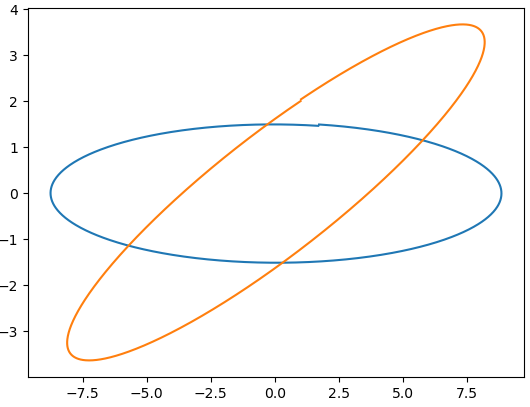
\includegraphics[scale=0.5]{section-06/qb-3.png}
        \end{center}
  \item \q{Après rotation de $\varepsilon$ et en la supposant symétrique par
          rapport à l'axe des $x$, calculer l'aire contenue dans l'ellipse
          $\varepsilon$ et vérifier que l'erreur avec la formule théorique est de
          0.4 \% pour }\il{N = 1 000}\q{ points.}

        \newpage
        \codeFromFileT{ressources/ellipse.py}{section-06/qc-1.py}
        \codeFromFileT{main.py}{section-06/qc-2.py}
        J'obtiens :
        \[
          \begin{array}{rcl}
            r & = & \il{0.047054748966392786} \text{\%} \\
          \end{array}
        \]

        \ul{Remarque :} J'obtiens bien une erreur de $0.4$\% pour
        \il{N = 10 000} et non \il{N = 1 000}...

\end{enumerate}
